%  chapter-03.tex

\chapter{Architecture}

In this chapter, we look at the architectural design our Rapid Recovery Desktop system. First, we explain the design decision involved in our architecture that is built on top virtualization, how this architecture fits with our threat model, and take a more detailed look at the structure of the trusted computing base. Next, we describe the design of virtual appliances, virtual machine contracts, and their recommended use with our Rapid Recovery Desktop system. Then, we describe the architecture of our virtualization security framework, called OSCKAR. Finally, we consider the architecture of our Rapid Recovery Desktop system, first from a file system perspective and then from a network perspective.

\section{Virtualization}

We chose to build our architecture using virtualization since it allows us to fundamentally change the security threat model and structure of the trusted computing base. Our threat model revolves around protecting user data and allowing the user to be in control of their system, even in the face of attack. While at the same time, giving the user reasonable recovery methods, such that they are not forced to chose between losing their personal data and getting their tasks done.

Virtualization also gives us a unique opportunity to restructure the trusted computing base of a desktop system. First, since a virtualization system provides a rich set of isolation properties, it can be used to effectively isolate a user's personal data. At the same time, a guest VM can be provided with a network file server mount point to give the user and applications the proper access to the data. Specifically, our FS-VM is a special network file server, which, using virtualization and virtual networking, is isolated and protected from attacks from both external malicious entities and internal services or applications that have been infected by malware. Next, placing applications into virtual appliances significantly reduces the threat they pose on user data, other applications, and the overall system. Also, since virtualization gives us the ability to easily and efficiently restore a virtual appliance to a known good state, we are able to restore an application to a working state in response to either a bad upgrade or a malware infestation. Better still, since the user's personal data is stored in the FS-VM, it is not lost in the virtual appliance recovery process.

Recall that virtual appliances are not in the trusted computing base and are considered untrusted. A virtual appliance is required to have a contract associated with it that allows the appliance access to precisely the privileges it needs. For example, it can have access to specific mount points on the FS-VM or perhaps none at all. Also, it may need access to only the external network or it might not need a network connection at all. Further, external network access can be limited to certain types of incoming or outgoing data. A diagram of this setup is shown if Figure\ref{fig:NetworkArchitectureSimplified}, we will extend this figure and explain it in more detail in section\ref{sec:NetworkArchitecture}.

\begin{figure}[tbp]
\begin{centering}
\rotcaption{The architecture of our Rapid Recovery Desktop from a simplified network view.}
\label{fig:NetworkArchitectureSimplified}
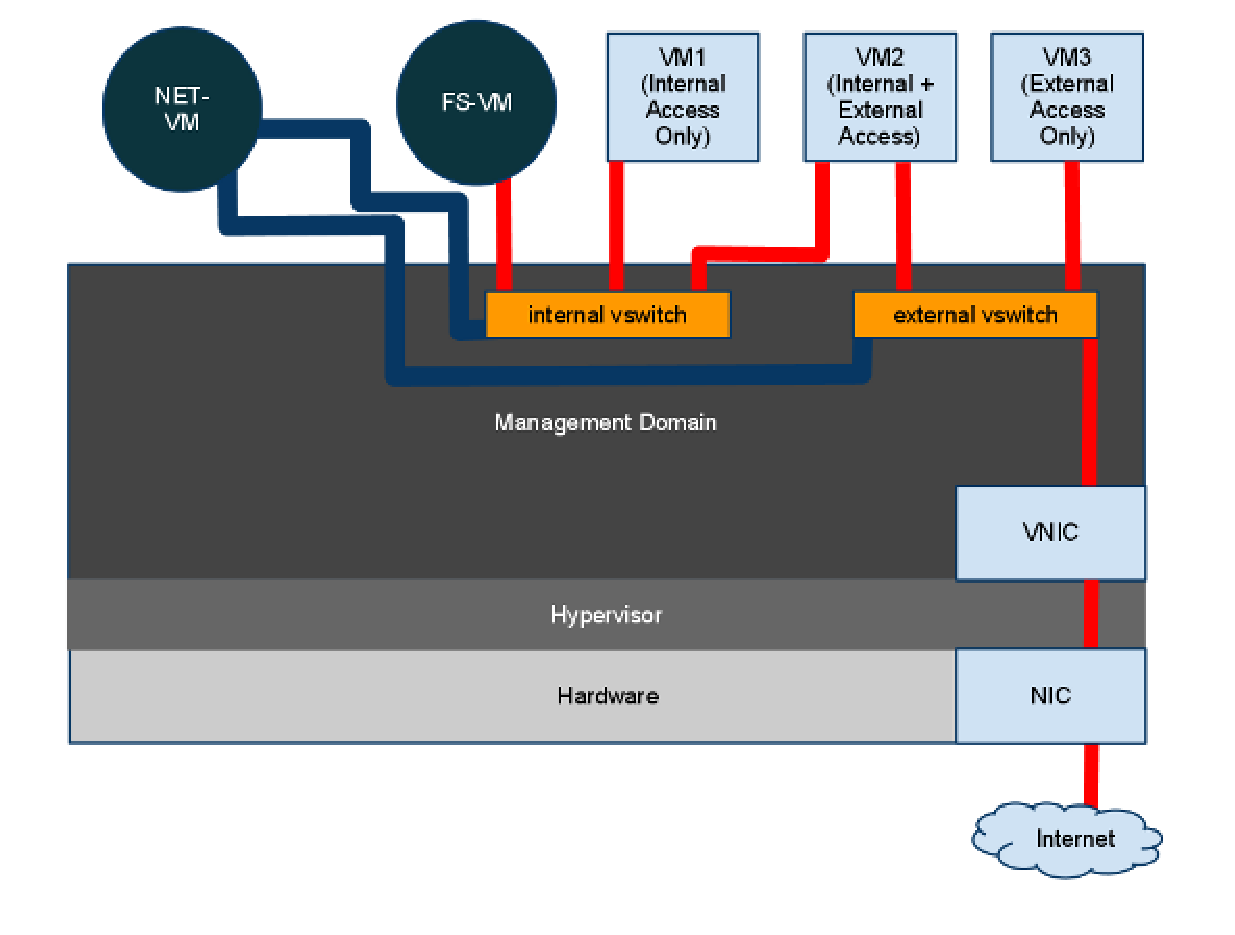
\includegraphics[scale=0.9,angle=90]{figs/NetworkArchitectureSimplified}
\end{centering} 
\end{figure}


With virtualization, we are also able to change the trusted computing base of the networking of the system. As needed, we are able to create a large number of isolated network segments within the same physical system. Based on our threat model, it is of utmost importance that we place our FS-VM on a virtual network segment that is not directly accessible from the outside Internet. In other words, an attacker must make two successful exploits in order to gain privileged access to user data. First, the attacker needs to compromise a virtual appliance that has been given access to the both the external network and some data on the FS-VM. Note that not all types of appliances need access to the external network, many appliances do not need access to the user's personal data, and some appliances (for example, local games) do not need access to the external network nor the user's personal data. Second, the attacker would need to use its position within the virtual appliance make a successful exploit of the highly protected and secured FS-VM. Only if an attacker was able to accomplish both of those exploits, would they be able to gain privileged access to the user's personal data. However, getting the data out without being detected and blocked would be the attackers next challenge. A closer look at the virtual network infrastructure, described next, shows why that task is also challenging.

As mentioned, since we are using virtualization, we can create a virtual network, which is built on a set of virtual switches that use an explicit allow and default deny policy to govern network accesses. The actual management of the switches is handled by our NET-VM component. This structure provides a layer of network defense, both from the outside Internet and the virtual appliances and other enforcement elements contained within the physical system, that significantly reduces the traditional attack vectors of malware and botnets. Malware that gains administrative access to a system will often first turn off network security systems, such as firewalls, anti-virus software, and intrusion detection systems. However, with the protection provided with our virtual switch network layer, turning off these defenses within the virtual appliance does not give the virtual appliance (nor the malware) any new access, since the network access policy is enforced from outside of the virtual appliance. 

Based on this virtual network layer, we turn back briefly to the attacker that has successful made two exploits to get to the user's data on the FS-VM. The FS-VM has no need to make outgoing connections (thus denied to do so by default), so even though the attacker is able to take control of the FS-VM and even to gain administrative access on it, they are unable to get it out of the system. The attackers only real hope is to find a lower level attack in the TCP/IP stack that could be used to exploit the NET-VM, then to change the networking policy to allow the FS-VM to connect out to the Internet. Note that making the first two exploits was unlikely in itself, further realizing the contraining enviroment and successfully making an exploit against it is much less likely. Research and development that defends against those type of lower level attacks is outside the scope of this dissertation. Lastly, we note that we are not arguing that an attack is not possible, but simply that an attack is made fundamentally more difficult with our architecture. We will describe the various types of malware behaviors and the correpsonding responses of our Rapid Recovery Desktop system in Chapter 5 on evaluation.

\section{Virtual Appliances}

A Virtual appliance, as described in section\ref{VirtualAppliances}, is one or more applications that are logically grouped into a virtual machine based on their network and data access needs. Notice that our definition of a virtual appliance is more specific than the traditional definition (any set of software installed within a virtual machine), so that our virtual appliances can be characterized by a single contract that is as specific as possible and integrated cleanly into the Rapid Recovery Desktop system proposed in this dissertation. There are many sites that offer pre-built virtual appliances for various virtualization platforms~\cite{vmware_appliances_website, rPath_website,  stacklet_website, virtual_appliances_website,  jumpbox_website}. Some of these virtual appliances may fit into our definition, but others are more general purpose appliances (e.g. full operating systems installed in a virtual machine) and are not well-suited for direct use with our system. Even the virtual appliances that are more specific don't have associated contracts, so contracts would still need to be written. In this section, we describe some specific examples of the types of virtual appliances that we recommend using with our Rapid Recovery Desktop system.

Our Rapid Recovery Desktop system can be configured in a variety of ways. We demonstrate that even in the most simple configuration, security benefits can be realized. We first show the security benefits with a single whole desktop virtual appliance. We then progress to our current recommended configuration, which is able to be setup on a wide variety of hardware and provides better security benefits at a small cost in terms of performance and complexity. We do not consider the more extreme configuration in which there is only a single application that runs in each virtual appliance, since we do not currently recommend this type of configuration, primarily due to current hardware and usability limitations. However, this type of configuration is something that we consider an important area of future work.

A simple configuration of our Rapid Recovery Desktop system would be to simply move a users complete desktop into a virtual appliance and configure it with a somewhat relaxed contract. This would allow users to have a nearly identical look and feel of their current system, but with some added security benefits. Specifically, some simple network contract rules, such as not allowing incoming connections, would provide significantly more protection than is commonly seen in practice today. More specifically, even in the face of attack, with an attacker gaining root access to the system and disabling the firewall on the operating system running in the virtual appliance, the network rules, since enforced outside of the virtual appliance would still provide protection. This defense alone would likely deter many would be attackers from extending their control over the system. For example, the attacker would not be able to easily make the compromised system part of a botnet, since it is not able to have access to an easy mechanism, such as an open port, to issue botnet commands to the virtual appliance. Notice that even with this simple case (moving a user's existing system, as is, into a virtual appliance and applying basic networking rules at the virtual network layer), we have significantly changed the playing field for attackers.

A next simple step to provide more protection and recovery to this simple configuration would be to move common data types, such as documents, photos, and any other files that are considered especially valuable to the user to the FS-VM and mount those files over the internal virtual network. This would allow for a more clear backup strategy. Specifically, backing up the FS-VM would backup files that are considered important to the user. Also, by capturing checkpoints of the virtual appliance, the full system could be easily rolled back to a known-good working state. Notice that this is a significant improvement over the alternative of rolling back a full system on a traditional desktop, since the user data would need to be backed up and restored manually by a user. It is also often more helpful and much more predictable than simply restoring only system files, as is done with a  traditional restore facility, such as Windows System Restore\cite{windows_system_restore}.

The alternatives, such as Windows System Restore, and full systems backups with tools like Clonezilla, and reset facilities such as Deep Freeze were discussed in related work. However, it is important to reiterate that the design of our system is complementary to having good backups, since the system only helps to make better backups and doesn't explicitly make backups of FS-VM data.  However, it does allow a user or administrator to create different backup strategies for user data and system data. Having mechanisms to backup the FS-VM could be enabled and are an area of future work. Also, other aspects of the design of our system make fine-grained restore of specific appliances possible. This aspect of the design is demonstrated by our recommended Rapid Recovery Desktop configuration option, described next.

The currently recommended way to configure our Rapid Recovery Desktop system is to have a set of virtual appliances that are as distinct as possible in their data and network access needs. For example, we recommend grouping applications that have similar data access needs and that may be used together to accomplish tasks. Grouping together applications such as browser-based applications and other internet-related programs, such as instant messengers, can be a good idea, since they all need a connection to the Internet and are likely to have fewer and similar access needs. Users will likely share similar types of information over various Internet-based applications. So, granting proper access to the types of files that they share over the Internet are likely to be similar. 

Another step would be to put each application into its own appliance. For example, email clients (not including web-based email, such as Gmail, Hotmail, or Yahoo! mail) may have a potential to fall in a similar class as Internet applications for some users, especially for users that use email infrequently or as a secondary communication method. However, it is likely that putting email clients applications in their own virtual appliance makes more sense, since there are many drive-by download type attacks on browsers that try to secretly install a small mail server to send spam. Thus, although having rules that restrict the amount of email from a combined Internet and email appliance could help, this wouldn't defend against more stealthy attackers that are willing to send spam email at a slower rate. So, having a separate email appliance makes contract rules simpler and provides a better level of isolation among applications. 

The two main drawbacks of a separate email appliance are that it requires more resources and that the data access patterns of Internet and email applications might be similar. If the system running our Rapid Recovery Desktop does have enough resources, we recommend having a separate email appliance, since the benefits are likely to outweigh the drawbacks. Future work sheds light on reasons why having separate virtual appliance, even with some overlap of data access needs, can be much more beneficial in terms of security benefits and the potential for better usability.

Other applications that make sense to group are applications that don't need any network access, such as many games and other personal-only programs, such as a diary application. In other words, anything that is not likely to be shared over the Internet with others. Highly sensitive applications, such as financial software, can be viewed similarly and can be grouped together, since this type of application needs to be protected well and should not need much, if any, data or network access needs. Any data that these sensitive applications would need to share with other remote entities or other appliances should be protected by contract rules. For example, if data from a financial application is needed by a document appliance for annual reports, then strict contract rules should allow for that specific access. Another scenario that a sensitive application, such as a financial application, would be a case where it needs temporary access to the Internet in order to get updates or to transfer information to or from a banking website. Handling such scenarios may require more complicated contracts or require special ways of doing things. More advanced contracts are an area of future work. Requiring extra effort on the user or appliance designer's part, although not desired, could be both acceptable and beneficial, as long as the users can clearly understand the security benefits gained.

Server software, although not necessarily common among desktop users, could become a lot easier to use and more secure when deployed as a virtual appliance in our Rapid Recovery Desktop model. Users could enjoy the benefit of having their own website or content management system without having to do much administration. Pre-packaged server appliances are common~\cite{vmware_appliances_website, rPath_website, stacklet_website, virtual_appliances_website, jumpbox_website}. Also server-based virtual appliances have well-known usage patterns and so writing virtual appliance contracts for web servers, database servers, and the like, is a much more straight forward process than trying to predict the usage patterns of desktop users. Further, breaking up the web server and database server components becomes easier and more attractive when it is integrated into the Rapid Recovery Desktop system architecture. For example, the database server could be accessed on a private network that is only accessible by the web server and only in very specify ways, such as only over a specific port. 

Let's take one example of a server-based virtual appliance, specifically a web server appliance. It would make sense to mount the web server's content to the FS-VM and grant read-only access to the web server appliance, so that even if the web server is compromised, the web site content is protected in the FS-VM. This method also allows for a more clear backup strategy and allows the web server appliance to be easily recovered. Write access to the web site data could be given to the appliance that handles creation and editing of that web data. In the case of content management systems, which often write there own data, contract rules that restrict the amount and type of data could be written to provide more protection than is typically bundled with a typical content management system.

Web server logs, unlike desktop operating system logs, can often be much more valuable from a user's perceptive, since measuring the usage of the server and types of visitors can be helpful. So, storing these types of logs in the FS-VM might be beneficial. Operating systems logs, while useful to system administrators, are not likely to be useful to the typically user. So, in general, users of our system can be smarter about the type of data that they consider to be valuable enough to backup more frequently and protect more carefully.

We have described examples of virtual appliance design here, while leaving out many of the details of actual implementation. In the next chapter (Chapter 4 on Implementation), we show more of the actual implementation details of a Rapid Recovery Desktop system that utilizes the design principles described in this chapter.

\section{Virtual Machine Contracts}

Virtual machine contracts (VMCs) are the glue that hold the system together. As described in the\ref{VirtualMachineContracts} section in Chapter 2, VMCs are starting to gain some research and standards-based traction\cite{virtual_machine_contract_ICAC09 }, but are not yet widely deployed in practice. For example, methods to assign more advanced network and data access needs within a VMC are not yet available. In this dissertation, we have designed and implemented a basic and generic virtual machine contract system that can be extended to support a wide variety of constraints on virtual appliances. The detailed design of VMCs is best addressed in the context of our virtualization security framework, which is described in the next section. Implementation details are then addressed in Chapter 4.

\section{Virtualization Security Framework}

To complement our decision to use virtualization, virtual appliances, and VMCs as the basis of our architecture, we needed to provide a communication mechanism for distributing the contracts to the various enforcement elements (for example, the FS-VM and NET-VM). For this purpose, we implemented a virtualization security framework, called OSCKAR. OSCKAR is structured as a message bus and policy management system that contains a set of interfaces that are used to interact with core components (for example, a VMM interface interacts with the hypervisor), enforcement elements (for example, an FS-VM interface interacts with the FS-VM), and control elements (for example, a Rapid Recovery Desktop interface interacts with the Rapid Recovery Desktop control component).

Note that OSCKAR only needs to contain core interfaces to function. It does not need to contain enforcement or control components to provide some basic functionality. For example, since the VMM interface is considered a core component, it must exist in OSCKAR's core functionality, which can then be used directly by a developer that includes the OSCKAR framework in their application. OSCKAR is designed to work with a variety of enforcement elements and control components. In this dissertation we focus specifically on two example enforcement elements, namely a NET-VM and FS-VM. We also present two examples of control components, namely the KIOSKAR control element (a simple virtual machine kiosk, described next) and the Rapid Recovery Desktop control element used to drive the functionality of the system presented in this dissertation.

The recommended use of the OSCKAR framework is for a product developer to extend OSCKAR to include a control interface that is used to interact with a control element that they create. A product that we developed to demonstrate this use case was a kiosk application, called KIOSCKAR, that allowed users to select and load a virtual machine from a graphical menu. The virtual machines available in the menu needed to be pre-loaded into the system by an administrator. To test OSCKAR's functionality, we created VMCs to be associated with each of the virtual machines. The virtual machines could be full operating system virtual appliances or special-purpose virtual appliances.

%would also like to somehow mention the statelessness of a kiosk and how we implemented it %with copy on write disks to store only temporary state, but explaining all the details of why % andhow makes it go too far off topic, maybe that will fit in another part of the dissertation    % better.

For our implementation of the KIOSKCAR product, we created a control interface library that connected to the OSCKAR core to provide high-level KIOSCKAR functions. A set of control elements were then created that interacted with the KIOSCKAR control interface. The control elements included a command line version of the kiosk, a window manager version of the kiosk, and a web-based version of the kiosk. Incidentally, the web-based version of the kiosk was developed by a sophomore communications major as a Clarkson Open Source Institute (COSI) project, which demonstrates that the high-level functionality of the KIOSCKAR control interface was reusable by other developers to provide a distinct user interface.

A more advanced product, which is demonstrated in this dissertation in the form of our Rapid Recovery Desktop system, makes use of all three types of interfaces, core, control, and enforcement. Our Rapid Recovery Desktop system uses the core VMM interfaces to interact with the hypervisor, it creates control interfaces to provide the basic Rapid Recovery Desktop functions, and it creates enforcement interfaces to interact with the enforcement elements (specifically the FS-VM and NET-VM). 

\subsection{Virtualization Security Framework and Virtual Machine Contracts}
With that high level description of the OSCKAR security framework, we now proceed with the design details of OSCKAR and describe how to associate a VMC with a virtual appliance using our OSCKAR framework. The implementation details of OSCKAR and specific examples based on real-world virtual appliances and contracts are show in Chapter 4. The architecture of OSCKAR is shown in Figure \ref{fig:OSCKAR}.

% http://www.ee.tamu.edu/~tex/manual/node37.html
\begin{figure}[tbp]
\begin{centering}
\rotcaption{The Achitecture of our OSCKAR Virtualization Security Framework}
\label{fig:OSCKAR}
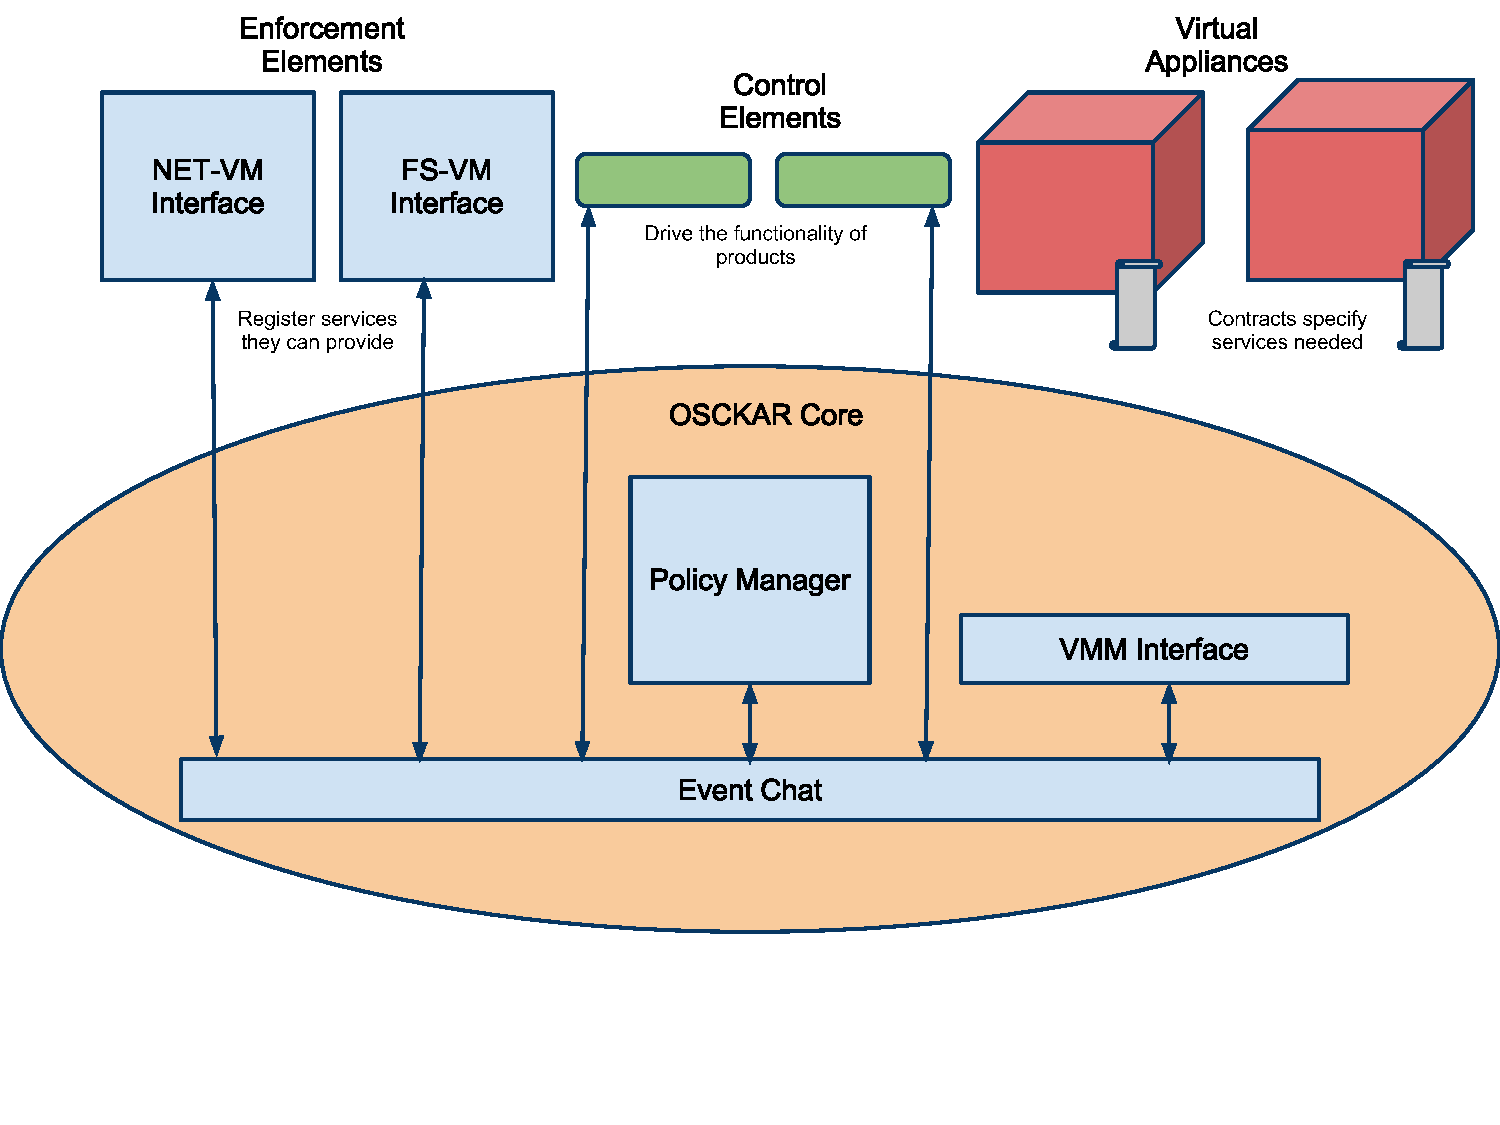
\includegraphics[scale=1.0,angle=90]{figs/OSCKARArchitecture}
\end{centering}
\end{figure}

At the heart of the OSCKAR architecture is a EventPolicy core, which is composed of two main components, an Event Chat message bus and a Policy Manager security daemon. 

The Event Chat component is a simple message bus and functions much like an Internet Relay Chat (IRC) server, in that it provides for authentication and communication among a Policy Manager (the trusted operator) and the various control and enforcement elements. The communication over the message bus is event-driven. Event Chat is designed to be simple, fast, and reliable. Our implementation of Event Chat uses a standard TCP socket interface, is multi-threaded, and is designed to receive a variety of input, even invalid input, and not crash.

The Policy Manager component is the security daemon. It implements the functionality of local and global policy, so that an administrator could have a global policy that would override a local contract policy. For instance, the administrator might want to disallow BitTorrent globally, even if a virtual appliance contract would otherwise allow it. The Policy Manger can also be configured to raise events in specific ways in order to better control operational logic. For example, when importing a contract, a portion of the contract may be used for building the disk image for the virtual appliance, this would be need to be sent to the builder interface before other steps, such as starting the VM, and so this type of sequential or dependency-based functionality is built into the configuration language of the Policy Manager.

At a high level, the EventPolicy core is designed so that it can also be used in other environments, such as event and policy management for home automation, and is not limited to use with virtualization. Our OSCKAR core component however is specifically designed for use with virtualization. Thus, we include a VMM interface inside of OSCKAR as a core component that interacts directly with the underlying hypervisor in an appropriate manner on behalf of OSCAR core. The VMM interface includes functionality to create, start, pause, suspend, restart, stop, and destory VMs.

In order to create a product, such as our Rapid Recovery Desktop, one or more control elements are necessary. Control elements are used to drive the functionality of the system. For instance, a control element for the Rapid Recovery Desktop needs to pass the virtual machine contract to OSCKAR, so that when the user wants to start the virtual appliance, the control element can instruct OSCKAR to start it. The same, or a distinct, control element could then be used to show the interface of the virtual appliance to the user.

Next, a product needs zero or more enforcement elements. Products can in fact exist without an enforcement element, As an example, consider our kiosk (the KIOSCKAR product described above), it booted virtual machines based on temporary stateless disks (changes to a copy-on-write disk image were destroyed when the virtual machine was shutdown) and did not require user data to be saved, so an FS-VM component was not necessarily. For security purposes, a NET-VM component could have been used, but putting the virtual machines behind a software network address translation (NAT) router and destroying state on every shutdown was sufficient security for an initial release. This is not to say that our kiosk product could not use enforcement elements, but adding enforcement elements, especially those used in our Rapid Recovery Desktop system, transforms the kiosk into somewhat of a different product. As the virtual machines that it boots become more like virtual appliance and the VMCs that protect the virtual appliances become more robust, the kiosk becomes more like a Rapid Recovery Desktop system with a kiosk front-end. An equivalent system would be to create a kiosk or web-based control element and interface for our Rapid Recovery Desktop system. This would be an interesting area of future work. 

The additional functionality that enforcement elements can provide make them an attractive option. For instance, an enforcement element for the Rapid Recovery Desktop system is the FS-VM component, which is used to allow specific virtual appliances, as specified in their contracts, to attach to specific data stores in order to provide file access control of user data. Similarly, our NET-VM component provides network access control for virtual appliances. Other enforcement elements can be added as needed and can then be used by virtual appliances by specifying the use of the enforcement element and rules in the virtual machine contract.

Since the communication over the Event Chat message bus is event-driven, control and enforcement elements simply register for and raise events that are filtered through the Policy Manger security daemon and handled by the appropriate elements. For example, the FS-VM in our Rapid Recovery Desktop product registers for the event ``mount\_documents'', then when a virtual appliance, such as a document editor, has a FS-VM rule that specifies a need to ``mount\_documents'', the request is passed through the Policy Manager component, to the FS-VM so that the processing can take place. Further, we require other FS-VM contract options, such as the access type (read, write, append, etc.) and allow other options, such as the rate of access, to be optional. In this manner, we put a lot of control on the FS-VM designer to build an FS-VM that is as powerful and flexible as they choose. We will further discuss other details of our control and enforcement elements in Chapter 4 on Implementation.

The control and enforcement elements are generic by design to allow their designers to provide as much or as little functionality as they choose and in the manner that they choose. For example, control and enforcement elements could be proprietary components that provide a similar service as our Rapid Recovery control element, FS-VM interface component, or NET-VM interface component. Control and enforcement elements could also be external physical components, such as a stand-alone firewall hardware appliance, that exists somewhere on the network. This flexible OSCKAR design is an example of providing an open source and open standards framework that can be built upon in innovative and competitive ways.

Finally, it is important to note that the OSCKAR virtualization security framework can be used for a variety of other products, not just our Rapid Recovery Desktop system. For example, as previously mentioned, during early development of Rapid Recovery Desktop, we developed a kiosk system, which we named KIOSCKAR. KIOSCKAR allows users to select from a menu of various operating systems, which are transparently run in a VM, and are able to use without needing to restart the computer. In other words, it is a operating system zoo running on a single computer. KIOSKCAR is open source and is being tested on some of the computers in the applied computing labs at Clarkson.

Other products that are either being worked on include an application segregation tool, called Appify, that will run ``appified'' applications in their own VM to provide for even finer-grained segregation of applications. Also, other ideas are that we could use OSCKAR to create a web-based VM administration tool, or a Virtual Desktop Infrastructure (VDI) management tool to provide desktop virtualization in the form of thin clients to a collection of computers, such as a classroom.

\section{File System Level Architecture}

In order to protect the user's personal data, portions of the file systems of the virtual appliances used in our Rapid Recovery Desktop system are mounted over a network file server (specifically our FS-VM). This allows us to restrict both the subset of data a virtual machine can access as well its access rights to that data. The specific portions of the file system that are mounted over to the FS-VM are appliance-specific. For instance, a browser appliance would likely mount the Downloads folder (typically \$HOME/Downloads in Linux and \$HOME/My Documents/Downloads in Windows) as read/write. Browser-specific settings and plugins could also be mounted on the FS-VM, if desired. A typical user may want to upload photos using their browser appliance, so the photos directory (typically \$HOME/Pictures in Linux and \$HOME/My Documents/My Pictures in Windows) should be mounted read-only. These mount rules and mount points would either need to be set up ahead of time by the virtual appliance designer and they should need to allow the user a way to configure them manually as desired. A photo editing appliance would want to mount the photos directory read/write, so that it could make modifications to the photos. This separation of privilege protects the user's photos from being corrupted by malware in the browser appliance. Having the data stored in the FS-VM also allows restoring the browser appliance to a known good state and leaving the user's data intact. The browser appliance would simply mount the data stored on the FS-VM on boot.

Although we do not focus on enhancements to the FS-VM in this dissertation , alternative FS-VM implementation can support a richer set of mount point permissions that allow ``write-rarely'' or ``read-some'' semantics as was shown in\cite{rapid_recovery_paper_05}. Specifically, an FS-VM designer could add read and write rate-limiting capability to each mount point in addition to full read or write privileges. Using this design, one can specify the amount of data that can be read or written per unit of time. For example, a mount point could be classified as reading at most 1\% of the data under the mount point in 1 hour. Such a rule could prevent malicious code from rapidly scanning the user’s complete data store. These read and write limits are just one example of a richer set of mount point permissions that can be used to help protect against attack. Append-only permissions (i.e. the ability to add new files but not modify or delete existing files) could be used to prevent removal or corruption of existing data. (SELinux has support for append-only file systems of this type\cite{smalley_2001}. For example, a directory containing photos could be mounted append-only in one virtual machine appliance allowing it to add photos, but not to delete existing photos. Another example would be restricting the size or file extension of files that are created (e.g. no .exe or files marked as executable files).

\section{Network Level Architecture}
\label{sec:NetworkArchitecture}

In this section we describe the virtual network design of our system. We set up three virtual switches (vswitches), namely an external vswitch, an internal vswitch, and an OSCKAR management vswitch. The external vswitch is connected directly to the physical network through the main network interface card (NIC) of the host system. The internal vswitch provides an isolated private internal network with no direct link to the external vswitch. The OSCKAR management switch is a private network that the OSCKAR framework uses to communicate over. All of the vswitches are managed by a NET-VM component. This architecture is depicted in Figure \ref{fig:NetworkArchitecture}.

\begin{figure}[tbp]
\begin{centering}
\rotcaption{The architecture of our Rapid Recovery Desktop from a network view}
\label{fig:NetworkArchitecture}
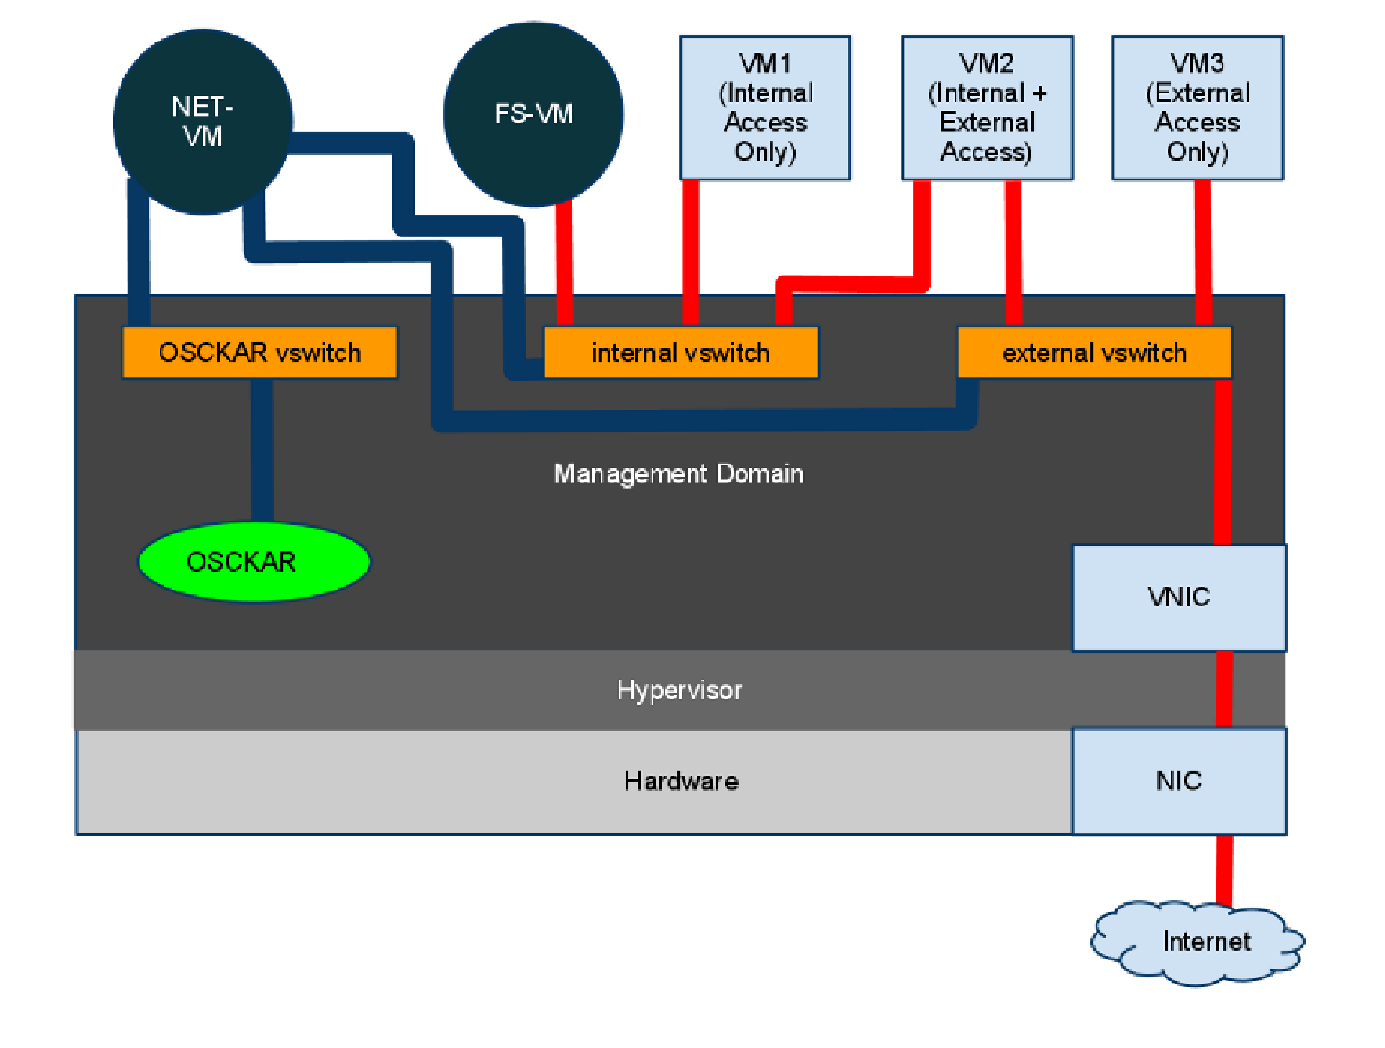
\includegraphics[scale=0.9,angle=90]{figs/NetworkArchitecture}
\end{centering} 
\end{figure}

This network design provides for logical isolation of the enforcement components and various virtual appliances, each of which can have differing network and data access needs. The most isolated component, the FS-VM, is connected to the internal vswitch and is only accessible to virtual appliances that have specified in their contract to have access to specific mount points of the FS-VM. This implies that an attacker would need to first exploit a virtual appliance and also then the FS-VM in order to gain access to user data. This architectural design alone is a significant improvement from the current traditional operating system model.

Next, the isolation of the external vswitch and the internal vswitch allow for logically different virtual appliances to have only the network and data access they need and no more. For example, it may be the case that a browser appliance only needs access to the external network and doesn't need access to user data stored on the FS-VM. Similarly, a photo or document editing program may only need access to specific mount points (photos and documents respectively) and not need any external network access. Finally, it may be the case that an email appliance needs access to documents and photos to save and send attachments as well as an external internet connection in order to send and receive email.

Finally, a network virtual machine (NET-VM) component is used to manage all of the vswitches. The NET-VM component is only given access to connect over a secure channel to a virtual switch management utility running in the management domain. This configuration allows logical separation of the NET-VM to the rest of the system and, similar to the protection of the FS-VM, provides isolation from attacks that target the network infrastructure. The NET-VM component could further be isolated by giving it exclusive access to the physical network card, which it would then have the vswitches within itself and act as a driver domain for the other virtual appliances that need network access. Advanced configurations, such as making the NET-VM a driver domain, will be discussed in the future work section of Chapter 6.

\subsection{Hardening the Overall System}

In this section, we discuss the basic design methodology of securing (or hardening) our trusted computing base. At a high level, we have enforcement elements, a virtualization security framework, a management domain and a hypervisor that are all considered part of our TCB. Recall that virtual appliances are not considered part of the TCB, but can benefit from general hardening strategies.

The basic hardening method that we employ is to keep things as simple as possible. For example, within the enforcement elements, such as the FS-VM, we remove all unnecesary services and keep the operating system to be as simple as secure as possible. This implies that no extra ports are open, a GUI is not installed if it is not needed, and modules are not loaded unless they are needed. We also suggest to use mandatory access control rules to protect the enforcement elements, both from the outside using a MAC embedded within the virtualization layer and within the VM itself using a standard MAC, such as SELinux or AppArmor.

Other strategies for hardening the system include using defense in depth and VM introspection techniques. Defense in depth means using a layered approach, for example by employing a firewall at the perimeter and also firewalls within. In practical terms this means that the base system should use a firewall as well as the VMs within it. Further, to protect the security software within the VM itself we suggest the use of VM introspection techniques. The basic idea is to inspect the critical code and data (for example on disk and in memory) of the VM from the hypervisor. We have not yet deployed this technique, but research and practical implementation work in this area will be discussed as part of the future work section in Chapter 6.

Finally, a key strategy that we employ to enhance the hardening is isolation. In particular isolating the various components onto their own network segments can reduce the surface area of attack. For example, the management domain and the virtualizaiton security framework can be isolated on their own isolated virtual network. A first pass implementation of this network architecture was described earlier in this chapter. In future work, we consider more advanced network control techniques, such as using a OpenFlow controller as the NET-VM component.

Now that we have described the design of our system, we move on to describing the implementation details in the next chapter.

